\citeauthor{Munzner2014} answers a lot of questions concerning the usage of visualizations in her book called "Visualization Analysis and Design". This chapter will discuss the most important answers because they are a necessity in understanding questions like when, why and how to visualize.

From today's perspective with the ability to use artificial intelligence and machine learning, the question if we still need a human in order to create visualizations is very valid. This questions as a very simple answer: if well-defined questions to ask about data exist in advance, it is possible to answer these purely with computational techniques from fields such as statistics and machine learning. If a solution to a problem has been fully automatized and has been deemed to be acceptable, there is no need for human judgement anymore and thus no need to design a visualization tool. An example for a practical application would be the domain of stock market trading. A tool in that field can be fully automatized currently there are many deployed systems for high-frequency trading. Those systems make decisions about buying and selling stocks when certain market conditions hold \iacite{Munzner2014}. Some other reasons where computers beat humans are mentioned below:
\begin{itemize}
\item Scale: Drawing a dataset of hundreds of thousands of items by hand is infeasible and would take a lot of time.
\item Efficiency: Once a problem has been solved with a computer it can be reused  indefinitely for different datasets and scenarios.
\item Quality: Precise data-driven rendering.
\end{itemize}
However many analysis problems are very poorly specified. Either the approach to the problem is unknown, or it is not obvious which questions the data could or should answer. In such a case, \citeauthor{Munzner2014} says, that the best path forward is an analysis process with a human in the loop. Even though there are a lot of use cases for a human in the loop, this paper only discusses one because it deals with \ac{EDA} (see chapter \ref{s:eda} on page\pageref{s:eda} for more information.), which is essential for this thesis. Exploratory analysis in scientific discovery is a common case of the need of a human. A long-term visualization tool which could be developed is a tool with the goal of speeding up and improving user's ability to generate and check hypothesis \iacite{Munzner2014}.

% Maybe use ability matrix here

Another important question answered by \citeauthor{Munzner2014} is: why depend on vision? As chapter \ref{s:definition} on page \pageref{s:definition} already mentions, a part of visualization is based on exploiting the human visual system as a means of communication. A significant amount of visual information processing occurs in parallel through high-bandwidth channels to our brain. One example \citeauthor{Munzner2014} mentions is visual popout: one red item in a sea of gray ones is immediately noticed.

Furthermore a single static view can show only one aspect of a dataset. This fact is already part of the answer of the next question: why use interactivity? Even though there are combinations of simple datasets and tasks where only a single visual encoding and therefore a single static view is needed, it does not apply for large complex datasets where interactivity allows to change displays and supports many possible queries. Interactivity could be used to investigate multiple levels of detail at once, ranging from a very specific detailed view of a small part to a very high-level summarization \iacite{Munzner2014}.

The main goal of a design of a visualization is to satisfy rather than optimize. One of the many possible good solutions to a problem is much harder to find than one of the even larger number of bad ones. Yet the validation of satisfaction is very difficult because there are so many questions considering wheter a visualization tool has met the design goals \iacite{Munzner2014}.

Furthermore it is needed to keep at least three different kinds of limitations in mind when designing or analyzing visualizatoins:
\begin{enumerate}
\item computational capacity,
\item human perceptual and cognitive capacity and
\item display capacity.
\end{enumerate}

All three limitations can be subsumized with the term scalability.

One of the most important questions \citeauthor{Munzner2014} answer is called: why analyze? In order to answer the question they feature an analysis framework that helps to think about design choices for visualizations systematically. Figure \ref{fig:an-framework} on page \pageref{fig:an-framework} shows the high-level framework they provide for analyzing a visualization's use according to three questions: what data does a user see, why does the user intend to use a visualization tool and how are the visual encoding and interaction idioms constructed in terms of design choices \iacite{Munzner2014}.

\begin{figure}[ht]
\centering
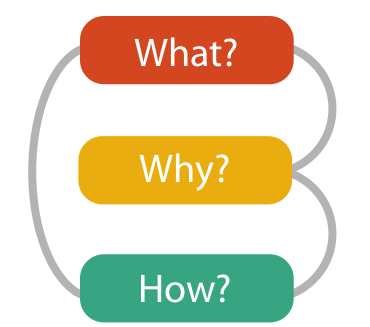
\includegraphics[width=0.3\textwidth,keepaspectratio]{images/basics/analysis-framework.png}
\caption[
    Three-part analysis framework for a visualization instance: why is the task being performed, what data is shown in the views, and how is the vis idiom constructed in terms of design choices \iacite{Munzner2014}.
]{Three-part analysis framework for a visualization instance: why is the task being performed, what data is shown in the views, and how is the vis idiom constructed in terms of design choices.}
\label{fig:an-framework}
\end{figure}